% !TEX TS-program = LuaLaTeX
\documentclass[11pt,compress,xcolor=x11names,UTF8]{beamer}
\usetheme{Boadilla}
\usecolortheme{seahorse}
\useinnertheme[shadow]{rounded}  
\useoutertheme[subsection=false]{smoothbars}
\usecolortheme{spruce}
\usecolortheme[named=SpringGreen4]{structure}
\usefonttheme{structurebold}
\useinnertheme{circles}
\usecolortheme{rose}
\usepackage{pifont}
\usepackage{academicons}
\usepackage{fontawesome}
\usepackage{iitem}
\usepackage{graphicx}
\usepackage{tabularx}
\setbeamertemplate{itemize item}{\ding{108}}
\setbeamertemplate{itemize subitem}{\ding{109}}
\setbeamertemplate{navigation symbols}{}
\setbeamercovered{transparent}  
\renewcommand\appendixname{附录}
\renewcommand\abstractname{摘要}
\graphicspath{{figure/}} % 图片路径
\usepackage{calligra} % Thank you
\usepackage{ctex} % 加入中文
%\setCJKsansfont{Noto Sans CJK SC}
\setsansfont{Lato} % Lato Roboto Fira Sans
\usepackage{makecell}
\newcommand{\tabincell}[2]{\begin{tabular}{@{}#1@{}}#2\end{tabular}}
\usepackage{url}					
\usepackage{natbib} % 参考文献
%\title[Spatial Generalized Linear Mixed Models]{Spatial Generalized Linear Mixed Models with Application to Prevalence Mapping}
\title{ Altnative way to Calibrate Light Field inside Drawers }
%\subtitle{奖助金申请答辩}
\author[Rong. Zhao]{Email:zhaor25@mail2.sysu.edu.cn \and  } % \\ 专业:统计学 \\ 方向:数据分析与统计计算
\institute[SYSU]{School of Physics\and } % 理学院\\
\date[\today]{
\includegraphics[width=.5\textwidth]{logo}}

\begin{document}

\maketitle

\begin{frame}{Outline}
\tableofcontents
\end{frame}

\section{Motivation}

%\subsection{研究意义}

\begin{frame}{about the container system}
%\textsf{例} \textbf{例}  \textit{例} 
% \texttt{例}  % 调出仿宋字体了
Currently, we calculate the PDE results of container by linearly mapping its internal PDE values to scanning station, which means the container is unable to give independent PDE values. 
%\begin{equation}
%PDE={\color{red}PDE_c}\cdot f_{cs}+constant
%\label{pde_cs}
%\end{equation}
%where  $PDE_c$ is the internal PDE result of container and  $f_{cs}$ is the correlation factor between two testing systems.\footnote{We believe the two systems are linear related.}

\vspace{.5cm}

\alert{The main reason is that we know little about the light field around the PMT surface.} 

\vspace{.5cm}

On the other hand, if we can measure the light field inside one drawer, it will become a powerful light source to evaluate PDE of PMTs. Suppose we know the incident photon numbers $n_i$ of one small area in the PMT surface $ds$, from scanning station could get the normalized PDE factor $P_i$ of this small area. Then we have   
\begin{equation}
\Sigma\limits_{i} n_i\times PDE\times P_i=n_{pe}
\label{eq:01}
\end{equation}
where $n_{pe}$ is the total output photon-electron number of PMT.
\end{frame}
%%%%%%%%%%%%%%%%%%%%%%%%%%%%%%%%%%%%%%%%%%%
\begin{frame}{The average PDE distribution}
%\vspace{.5cm}
The factor $P_i$ is from the average PDE map of PMT cathod, which is based on scanning station's results\footnote{hang hu \rightarrow https://juno.ihep.ac.cn/cgi-bin/Dev\_DocDB/ShowDocument?docid=3665}

\begin{figure}
\centering
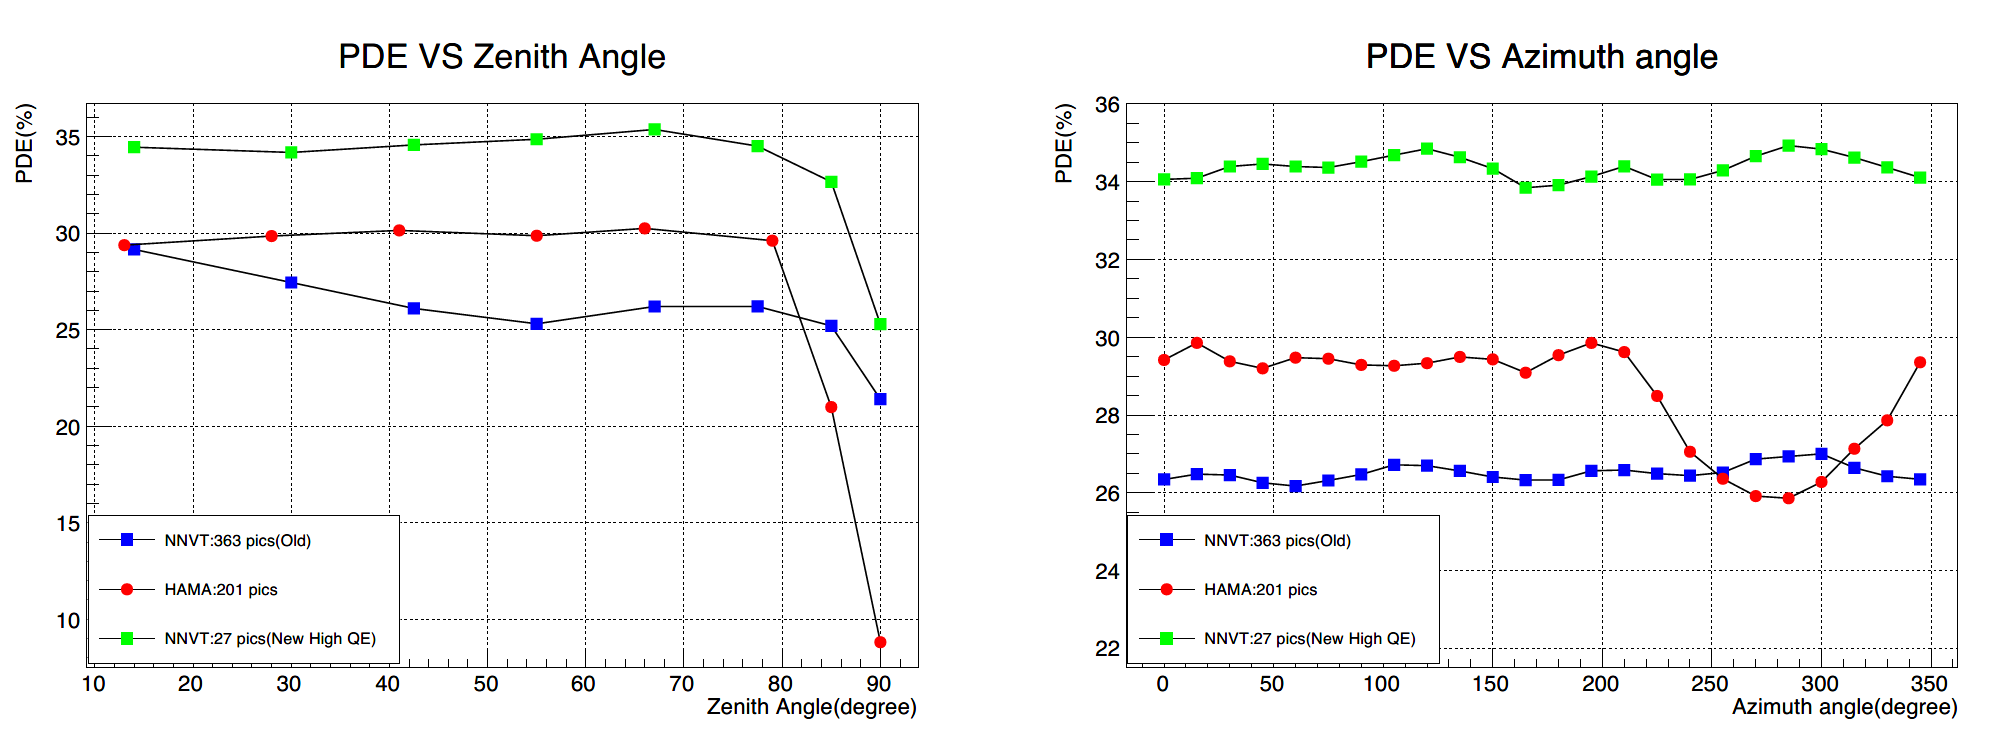
\includegraphics[width=0.98\textwidth]{pdecathod} % 单图
\caption{average PDE on cathod from SS}
\end{figure}

\end{frame}
%%%%%%%%%%%%%%%%%%%%%%%%%%%%%%%%%%%%%%%%%%%
\begin{frame}{calibration methods}
From equation\ref{eq:01} we have:
\begin{equation}
PDE=\frac{n_{pe}}{\Sigma_{i} n_{i}\times P_{i}}
\end{equation}

The PMT cathod is divided into $8\times 24$ parts in the SS system, so it is reasonalble to apply the same scheme when measure light field. 

\vspace{.5cm}

The item $\Sigma_{i} n_{i}\times P_{i}$ is exactly the $drawer_{factor}$, the advantage of this method is that we know what the light filed is and how PMT response to it.

\vspace{.5cm}

Apart from this discrete scheme, we can also perform finer light field calibration by measuring more points on the cathod and interpolating the PDE average map.

\end{frame}
%%%%%%%%%%%%%%%%%%%%%%%%%%%%%%%%%%%%%%%%%%%
%\begin{frame}{calibration of each drawer}
%Generally, we put several PMTs with known PDE value\footnote{or QE value}  into one drawer and linearly fit the PDE-$\mu_{test}$ data to get \alert{drawer$_{factor}$}. 
%\vspace{.5cm}
%\hrule{\textwidth}
%\vspace{.5cm}
%
%While an alternative way to access the drawer$_{factor}$ is fitting PDE-$\mu_{test}$ data {\color{red}from all the PMTs tested in one drawer rather than the mannual selected ones.} Then once we finish one PMT test in a drawer we will get one more statistical sample in the PDE-$\mu_{test}$ fitting, and we could expect that the fitted drawer$_{factor}$ will get more stable as we testing more PMTs.
%
%\vspace{.5cm}
%The advantage of this "self-calibration" method is that we could {\color{red}decrease the statistical error as much as possible}; and the remained fluctuation of drawer$_{factor}$ can be the system error. 
%\end{frame}
\section{possible  methods to achieve the calibration}
%%%%%%%%%%%%%%%%%%%%%%%%%%%%%%%%%%%%%%%%%%%
\begin{frame}{possible  calibration methods}
Below are the possible method to achieve the measurement:
\begin{itemize}
\item small semiconductor photo detector(like PD).
\item use HAMAMATSU 20" PMT with only small part(depend on the PDE map we have) exposed to the light, use the PDE map to determine light field. 
\item Set a strong light source and measure the saturation current as  a relative light field distribution\footnote{suppose QE is uniform along the cathod}.
\end{itemize}
\end{frame}
%%%%%%%%%%%%%%%%%%%%%%%%%%%%%%%%%%%%%%%%%%%
%~~!!!!!!!!!!!!!!!!!!put two figures to illustrate!!!!!
\section{summary}

\begin{frame}{summary and conclusions}
\begin{itemize}
\item This light field measurement is a finer version of drawer calibration, when combined with the PDE map from SS, we could know more about the PDE of one PMT.

\item If the container and scanning station use similar method to evaluate PDE of PMTs we could expect better consistency between these two testing systems. 

\end{itemize}
\end{frame}

\begin{frame}{summary about the DAQ learning}
I was onsite from Oct 27th - 31th, learning the operation, basic components and trouble shooting of container system. \\
\vspace{.5cm}
\hrule{\textwidth}
\vspace{.5cm}
Now, I am able to  
\begin{itemize}
\item daily maintenance, such as modifying testing parameters to meet our testing needs.  
\item update or replace the hardware components.
\item remotely help the onsite container expert to try to address the potential problem when system  not running properly.
\item onsite trouble shooting when severe problem happend.

\end{itemize}
%onsite container expert$\rightarrow$ seek help from rong or haiqiong remotely$\rightarrow$

\end{frame}
%%%%%%%%%%%%%%%%%%%%%%%%%%%%%%%%%%%%%%%%%%%
\begin{frame}{The  flow diagram of handling DAQ problem}
\begin{figure}
\centering
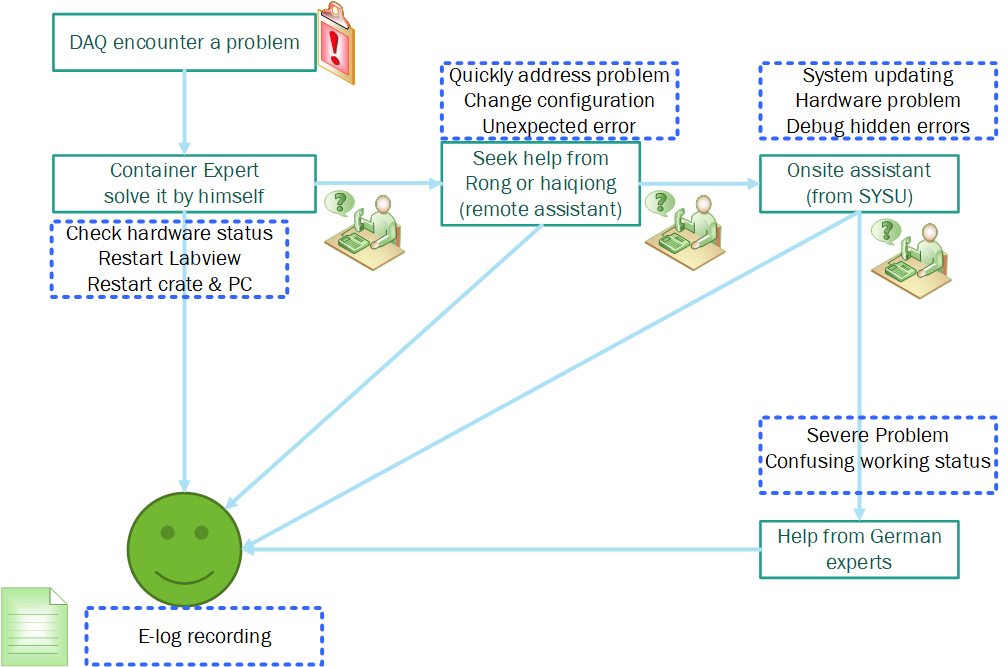
\includegraphics[width=0.9\textwidth]{daq} % 单图
%\caption{average PDE on cathod from SS}
\end{figure}

\end{frame}

\begin{frame}
\centering {\zihao{0} \color{red} \calligra{BACK-UP}}
\end{frame}

%\begin{frame}[allowframebreaks]
%\frametitle{References}
%\scriptsize
%\bibliographystyle{authordate1}
%\bibliography{R-GLMM-pkgs}
%\end{frame}

\appendix

\section*{附录}

% library(R2OpenBUGS) # 2017-2-20 version 3.2-3.2
% library(R2WinBUGS) # 2015-07-29 version 2.1-21
% library(rjags) # 2016-02-19 version 4-6
% library(BRugs) # OpenBUGS 2017-06-26  version 0.9-0
% library(glmmBUGS) # Generalised Linear Mixed Models with BUGS and JAGS 2016-09-22 version 2.4.0
% library(R2jags) # Using R to Run 'JAGS'  2015-08-23	 version 0.5-7

% network
	% diagram DiagrammeR DiagrammeRsvg
 % library(help=graph)

 % library(help=Rgraphviz)
 % library(help=igraph)


%\begin{frame}{Ack}
%\begin{itemize}
%\item[\faGithub] \href{https://github.com/Cloud2016}{Cloud2016} \faAt Github
%\item[\aiOverleaf] \href{https://www.overleaf.com/}{Xiangyun} \faAt Overleaf
%\item[\aiarXiv] \href{https://arxiv.org/}{arXiv}
%\end{itemize}
%\end{frame}

\end{document} 


